\documentclass[12pt,twoside]{article}
\newcommand\tab[1][1cm]{\hspace*{#1}}
\usepackage{pdfpages}
\usepackage[utf8]{inputenc}
\usepackage{graphicx}

\usepackage{verbatim}
\begin{document}
	
	\newpage
	\tableofcontents
	
	\newpage
	
	\section{General Introduction And Motivation}
	\pagenumbering{arabic}
	\par Project is about developing a standard representation for storing and sharing MathData, in the form of the description language
	MathDataLanguage. By providing a unified and publicly accessible MathDataLibrary, we expect that the communities of both
	mathematicians and computer scientists will embrace the new standard and take advantage of it. Building on this new data
	representation, we develop a fully automated system for performing benchmarks, called BenchIT. The benchmarks are shareable,
	reusable and reproducible, because they are expressed in a descriptive language that is independent of the scientific area, the
	hardware platform or the software used. This way, BenchIT can reproduce all the tasks necessary in any given environment fully
	automatically. This breaks the barrier that for many scientists, who are not familiar with computer science, prevents them from
	performing benchmarks and sharing their experimental results. Following the paradigm of web platforms for sharing hardware
	benchmarks, we provide a web platform for sharing software benchmarks. Such a platform would be useful for industrial users who
	wish to evaluate new software solutions without the overhead cost of performing a resource consuming evaluation of the available
	solutions. The approach we take is to design the data description language covering the 5-fold representation (see section 4) and a
	related repository structure to store MathData. We use existing standard tools such as git, in order to version control the data in an
	advanced way to avoid redundancy and respect the mathematical context and features of the data. 
	The goal of the project is to have a system for storing, retrieving and searching MathData in a consistent and robust way. 
	This system can be used either locally by the user or online as a service. 
	For the local version, a JupyterLab is provided. Since JupyterLab is a standard tool in data science, the intension is to incorporate MD in the standard data science workflow.
	\par We want to have a uniform language for describing math data and benchmarks. 
	This language is based on json. There are many different ways of representing data. And there are many different aspects of data.
	We want to cover these in a uniform way. On top of that, we want everything to be immutable and reproducible. 
	Thus version control is used. 
	
	Everything (mathdata, benchmarks, etc)stored in a git repository and it is referred to by a SpeceTime object. SpaceTime specifies the url of the git repo and the revision in which the stored information was committed. 
	
	%We have 5 aspects of data that we take into account:
	
	%\begin{itemize}
	%	\item raw representation
	%	\item typeset
	%	\item semantics
	%	\item context
	%	\item features
	%\end{itemize}

	
	\section{FUNCTIONALITY}
	
	
	\par If the repo file reach the limitation, new repo file should be created under raw directory.  
	
	
	Instances.txt;
	
	\{ \newline
	  \tab "raw" : KR, \newline  
	  \tab "typeset": KT,  \newline
	  \tab "semantics": KS, \newline
	  \tab "context": KC, \newline
	  \tab "features": KF, 
	
	\} KI  \newline
	
	Index.txt file is holding the key of Instances key. Also, If the raw or other data key change then new instance key is created. Even if the changed key removed. 
	      	
	Even if the key removed from index.txt, it still will be in database.
	Index.txt. It is being held to know what is in database. Also, User will reach removed key data over this key.
	
	
		
		 -------- Benchmarks and datasets are reading data from instances.txt and sending getindex or listindex to others? to do their task over index.txt ?? ------
		
		
		When user press the button over interface for the keys, retrieve function runs and this function retrieve 5-fold representation from instances.txt. 

		
		\par When the raw key or other datas key are updated, the instance key should be changed according to data changes. But the previous key should be kept in index.txt to show context to the user.
		
		Raw, context, semantics, typeset and features are sending as a string from front-end to back-end.
		Mdata language to semantics and typeset options 
		To mdatalanguage json context and raw 
		Backend to frontend sha keys
		
		Everything should be valid so job file will use and files can extend more and more .

		
		There is a .Json file for every context type such as polynomial.json, list.json graph.json etc.
		
	
		Updating and removing operation is done with index.txt when searching is done over instances.txt.
		
	\section{INTERNAL CAPABILITIES}
	
	
	\newpage
	\section{APIs}
	
	\subsection{MathData Restful}
	
	\subsection{Benchmarks}
	\par The MDB consists of the following parts:
	\begin{itemize}
		\item The mathdatabase python package.
		\item The mdb-server
		\item The mdb-interfaces
	\end{itemize}
	
	\subsection*{mathdabase python package}
	\par The python package provides all necessary commands for manipulating the mdb. Note that not all of these functions will be exposed to the user.
	
	\subsection*{mdb-server}
	\par The mdb-server provides a restful API to communicate the mdb. 
	The server imports the mathdatabase python package and interacts with the database through it.
	The server receives http requests and responds json objects in a RESTful way.
	
	\subsection*{mdb-interface}
	\par The mdb-interfaces are different interfaces for the mdb. 
	Some of them are:
	\begin{itemize}
		\item Jupyter-extension
		\item python package mathdata (which is different from mathdatabase, since it only exposes user accessible functions)
		\item MathDataLibrary website (this is our website with our custom design)
	\end{itemize}
	
	\par Other interfaces can be created for sage, Mathematica, Maple, Matlab, etc.
	
	\section{DATABASE STRUCTURE}
	
		
			
	\section{MATHDATA LANGUAGE}
		\par The MD-language is a DSL (domain specific language) for describing mathematical data.
		Mathematical data means structured data together with a context.
		The MD-language consists of a set of keywords and a specification for what the value of each keyword can be.
		
		\begin{figure}
			\centering
			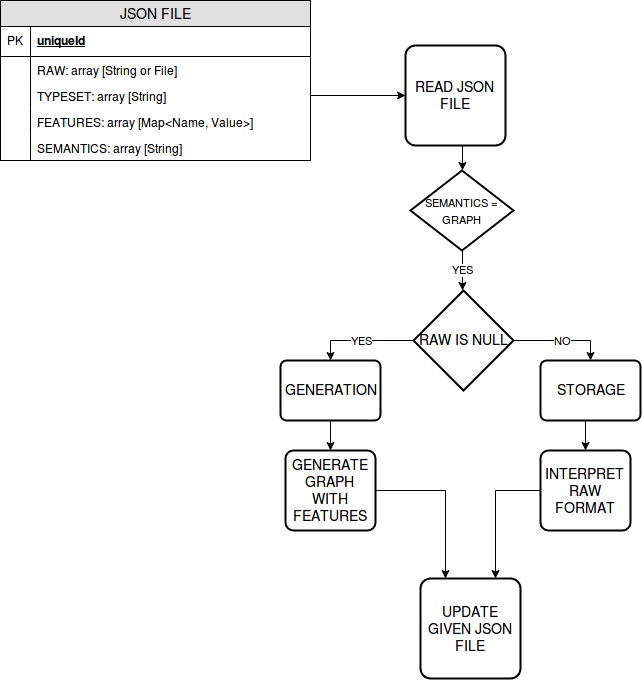
\includegraphics[width=\linewidth]{figures/mdlanguage.png}
		\end{figure}
		
		\subsection*{Specification of MathData}
		\subsubsection*{Keywords}
		We need the following keywords in order to specify new datatypes:
		
		\begin{itemize}
			\item list
			\item set
			\item singleton
			\item matrix
			\item structure
			\item element
			\item label (nodes, edges, variables etc.)
		\end{itemize}
	
		
	\newpage
	%\subsubsection*{Composing Types}
	%\par When designing a new datatype, we can use in the specification of the new datatype as values existing datatypes. These are called known datatypes and are %registered in the datatype registry of the MathDataLibrary.
	%For example, if a datatype \textcolor{red}{Integer} is registered in the MathDataLibrary, we can have in the specification of the new datatype the following:	
	%\newline
	%\begin{figure}[!h]
	 %\includegraphics[width=1.2\textwidth]{cap1.JPG}
	%\end{1figure}
	
	\par
	%Let's define the datatype \textcolor{red}{Graph}:
	
	%\begin{figure}[!h]
	%	\includegraphics[width=1.2\textwidth]{cap2.JPG}
	%\end{figure}

	%if the datatype \textcolor{red}{Graph} is registered, then we can have in the specification of \textcolor{red}{DynamicGraph} the following:
	
	%\begin{figure}[!h]
	%	\includegraphics[width=1.2\textwidth]{cap3.JPG}
	%\end{figure}

	%\subsubsection*{Inheritance}
	%	New datatypes can be created by inheriting from other (registered) datatypes. 
	%	For example, a tree is a graph with special properties.
	\section{BENCHMARK LANGUAGE}
	
	\section{CASE STUDIES(existing datatype definitions and benchmark definitions)}
	
	Wiki - > TERMINOLOGY
	
	\section{The MathDataLibrary}
	
	\section{The MathBenchmarkCentral}
	
	
	\section{LIMITATIONS}
	
	\section{DESIGN DECISIONS}
		\subsection*{Back-End}
		What goes in index.txt: \newline
		\{ \newline
			\tab "raw": SHA1, \newline
			\tab "semantics": SHA2, \newline
			\tab "typeset": SHA3, \newline
			\tab "context": SHA4, \newline
			\tab "features": SHA5, \newline
		\}
		
		\begin{figure}[!ht]
			\centering
			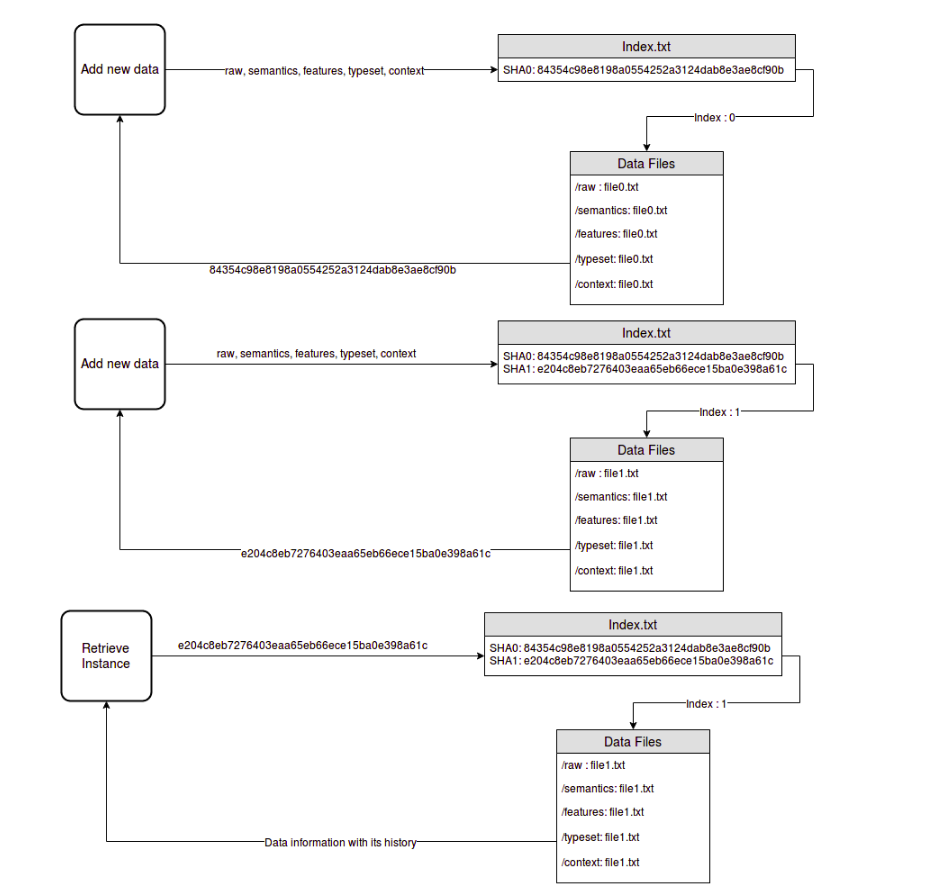
\includegraphics[width=0.7\textwidth]{figures/Scenario1Backend.png}
		\end{figure}
		
		\begin{figure}[!ht]
			\centering
			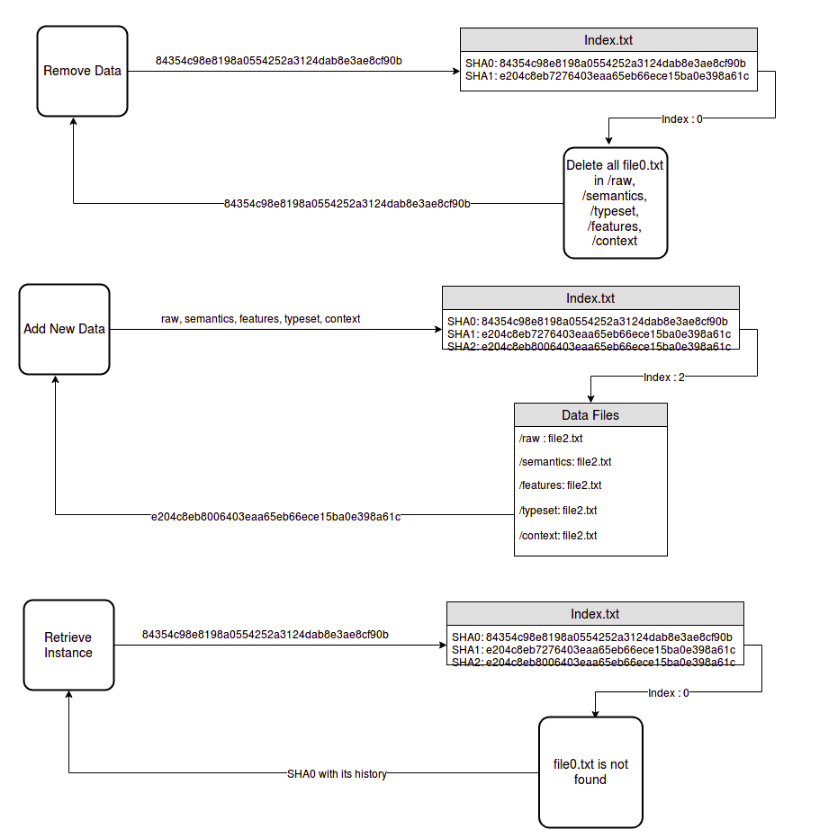
\includegraphics[width=0.7\textwidth]{figures/datadelete.png}
		\end{figure}
		
		
		\subsection*{Jupyterlab Extension}
		
		\subsection*{Restful API}
		
		\subsubsection*{Restful API}
		
		\par Restful Web Servisces are basically REST Architecture based web services. In REST Architecture everything is a resource. Restful web services are lightweight, highly scalable and maintainable and very commonly used to create APIsfor web-based applications.Rest uses HTTP protocol for data communication.It revolves around resources where every component is a resource and resource is accessed by a common interface using HTTP standard methods. A restful web service usually defines a URI,which is a service that provides resource representation such as JSON and a set of HTTP Methods.
		
		\subsubsection*{Flask}
		
		\par Flask is lightweight, micro web framework for python. The goal is to keep the core simple but extensible. Flask won't make many decisions for us such as what database to use or what template engine to choose. Flask also has extensive documentation that address everything that developers need to start. Microframework refers to a lightweight web application framework in contrast to full-stack frameworks. That means Flask gives only what we need essentially to create a back-end server but provides the flexibility to install any extensions to support features like protection and so on. Flask is a very good option for developing RESTful APIs.
		\newline \newline
		Flask-restful is extension of the flask that can install with,
		\newline
		\tab \textit{pip install flask-restful}
		
		
		
		\subsubsection*{Jinja2}
		
		\par Jinja2 is a template engine, on which flask is based. Instead of returning hardcore HTML from the function, a HTML file can be rendered by the render\_template() funtion. A web template contains HTML syntax intersperted placeholders for variables and expressions which are replaced values when the template is rendered. All we have to do is provide the name of the template and the variables we want to pass to the template engine as keyword arrguments.
		\newline\newline
		Jinja2 is installled with flask-restful installation automatically.
		
		\subsubsection*{Webapp}
		
		\par System starts with start function using flask route() function which is a  decorator tells the application which url should call the associated function.Start function enables the HTTP methods to data operation.
		
		\begin{itemize}
			\item add\_instance: route is a flack decorator to specified that server will be listening /add\_instance URL. New instance's request type specified with json then this instance is added to mdb via database.io. Return value that is type python is converted to json type with flask's json.dumps()
			\item ...
		\end{itemize}
		 
		
		\subsection*{MD Language}
	
	\section{STYLE GUIDE}
	
	\subsection*{Function Names}
	\begin{itemize}
		\item words separate with underscore. An example "first\_example"
		\item numbers are not separated with underscore. An example "new\_repo3"
		\item only lowercase letters can be used.
	\end{itemize}
	
	\subsection*{Comment Style}
	
	\subsection*{Module Organization}
	\section{FUTURE PLANS - TODO}
		\begin{itemize}
			\item Dataflows and Analytics with juttle
			\item BibManager
		\end{itemize}
	
	
\end{document}